

\section{Experiments}

%\subsection{Hello World}

In this section, we delve into the experimental core of our study, systematically addressing six critical questions surrounding model merging in the context of pre-training: 1) How does model merging affect  performance? 2) How do different merging methods affect final performance? 3) How to determine the optimal interval and number of weights to merge for various model sizes? 4) Do merged pre-trained models contribute to better downstream training? 5) Does model merging improve the stability of training? 6) What processes unfold during model merging? Through these experiments, we aim to provide comprehensive insights into model merging, offering practical guidance for its application and shedding light on its theoretical underpinnings.

\subsection{How does model merging affect model performance?}
Current learning rate schedule methods mainly involve constant learning rates or cosine annealing. In our model pre-training, we employed the Warmup-Stable-Decay (WSD) strategy~\cite{hu2024minicpm}, which combines a constant learning rate phase with a subsequent cosine decay phase~\cite{loshchilov2016sgdr}. To explore the effects of model merging under different learning rate schedules, we conducted experiments during both constant learning rate phase and cosine dacay phase.

In the constant learning rate phase, we merged fully trained models of various sizes. As shown in Figure~\ref{fig:overall}, the merged models exhibited significant performance improvements across multiple downstream tasks. For example, on the Humaneval benchmark, Seed-MoE-1.3B/13B improved from 31.1 to 36.6 points, and Seed-MoE-10B/100B increased from 54.3 to 61.6 points. While larger models showed less pronounced gains on certain benchmarks, such as BBH, this was likely due to the near-saturation of these metrics. Overall, the improvements were robust and consistent across model sizes.

Next, we performed model merging in the cosine annealing phase by collecting weights from the annealing stages of Seed-MoE-1.3B/13B, Seed-MoE-10B/100B, and Seed-MoE-15B/150B. As depicted in Figure~\ref{fig:aneal}, as the learning rate gradually decreased, the models converged steadily, with performance continuing to improve. Interestingly, at the early annealing stage, the results of ~\OURS{} were comparable to those at the end of the annealing process. In some cases, particularly for larger models, the merged models even surpassed those naturally annealed.

\begin{figure}[h]
    \centering
    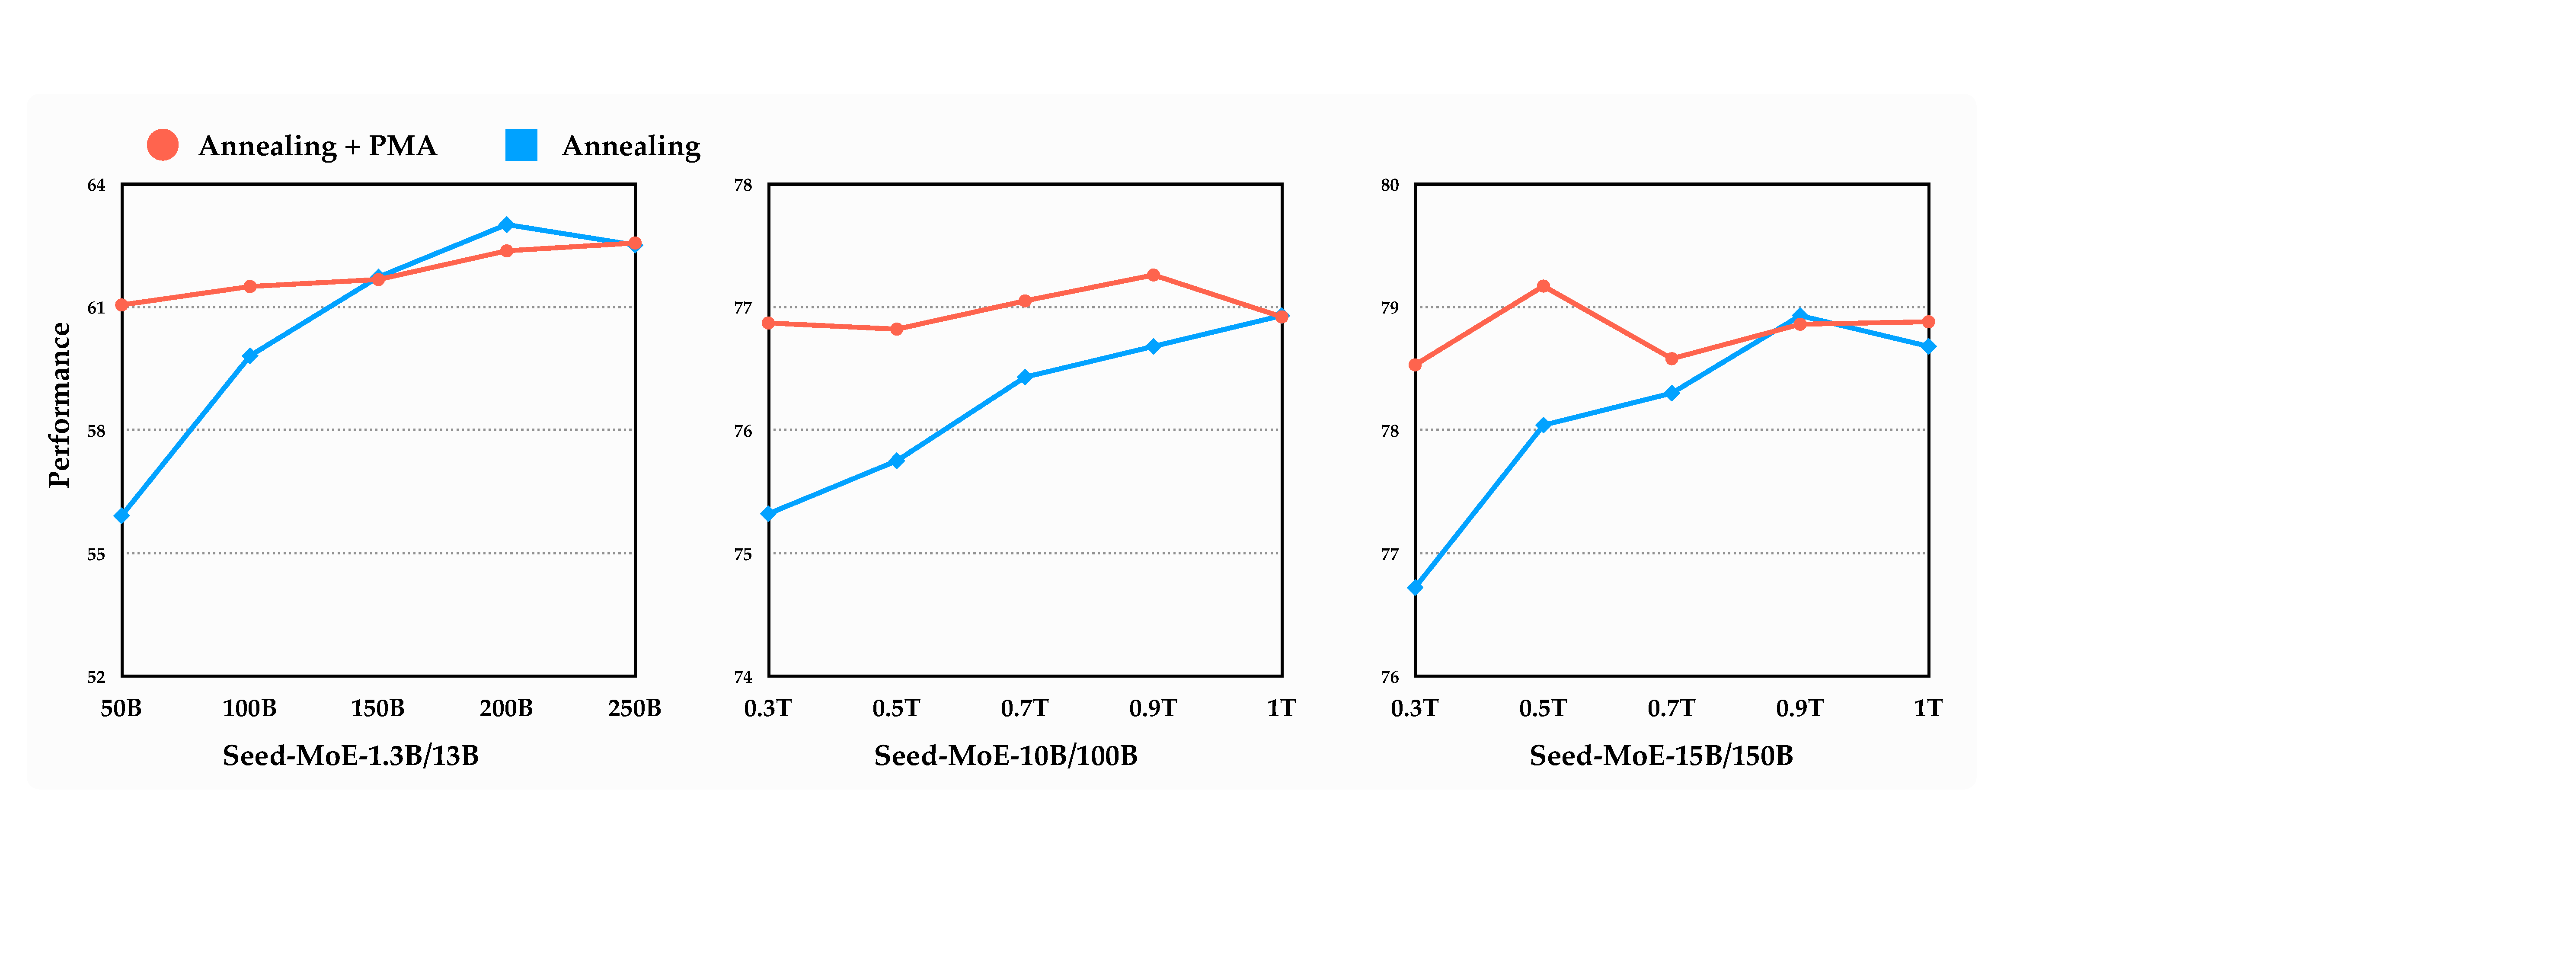
\includegraphics[width=0.9\linewidth]{image/aneal.pdf}
    \caption{Comparison of overall performance for MoE models of varying sizes under annealing training, before and after model merging. The learning rate follows a cosine schedule during the annealing process. The x-axis shows the count of training tokens.}%\CY{How about we use "$\texttt{WSD}_{cosine}$" or "$\texttt{Annealing}_{cosine}$" to replace the "\texttt{Annealing}" in figure legend, and relevant texts? }}
    \label{fig:aneal}
\end{figure}
These findings raised a question: could we simplify the training process by using only the Warmup-Stable phases alongside \OURS{}, skipping the decay phase, and avoiding learning rate adjustments? To investigate, we forked two training runs from the stable phase of Seed-MoE-1.3B/13B at 1.4T tokens. One continued with a constant learning rate, while another underwent annealing, each training for an additional 250B tokens. We then merged the models trained with the constant learning rate. As shown in Figure~\ref{fig:cons_vs_aneal}, early in training, the merged models significantly outperformed both the constant learning rate and annealed models. Even later, their performance was comparable to the annealed models.

This suggests that \textbf{pre-training with a constant learning rate, combined with model merging, can effectively match the performance of an annealed model at any point in the training process without the need for learning rate annealing}. This approach accelerates model validation and significantly reduces computational resource demands.

\begin{figure}[h]
    \centering
    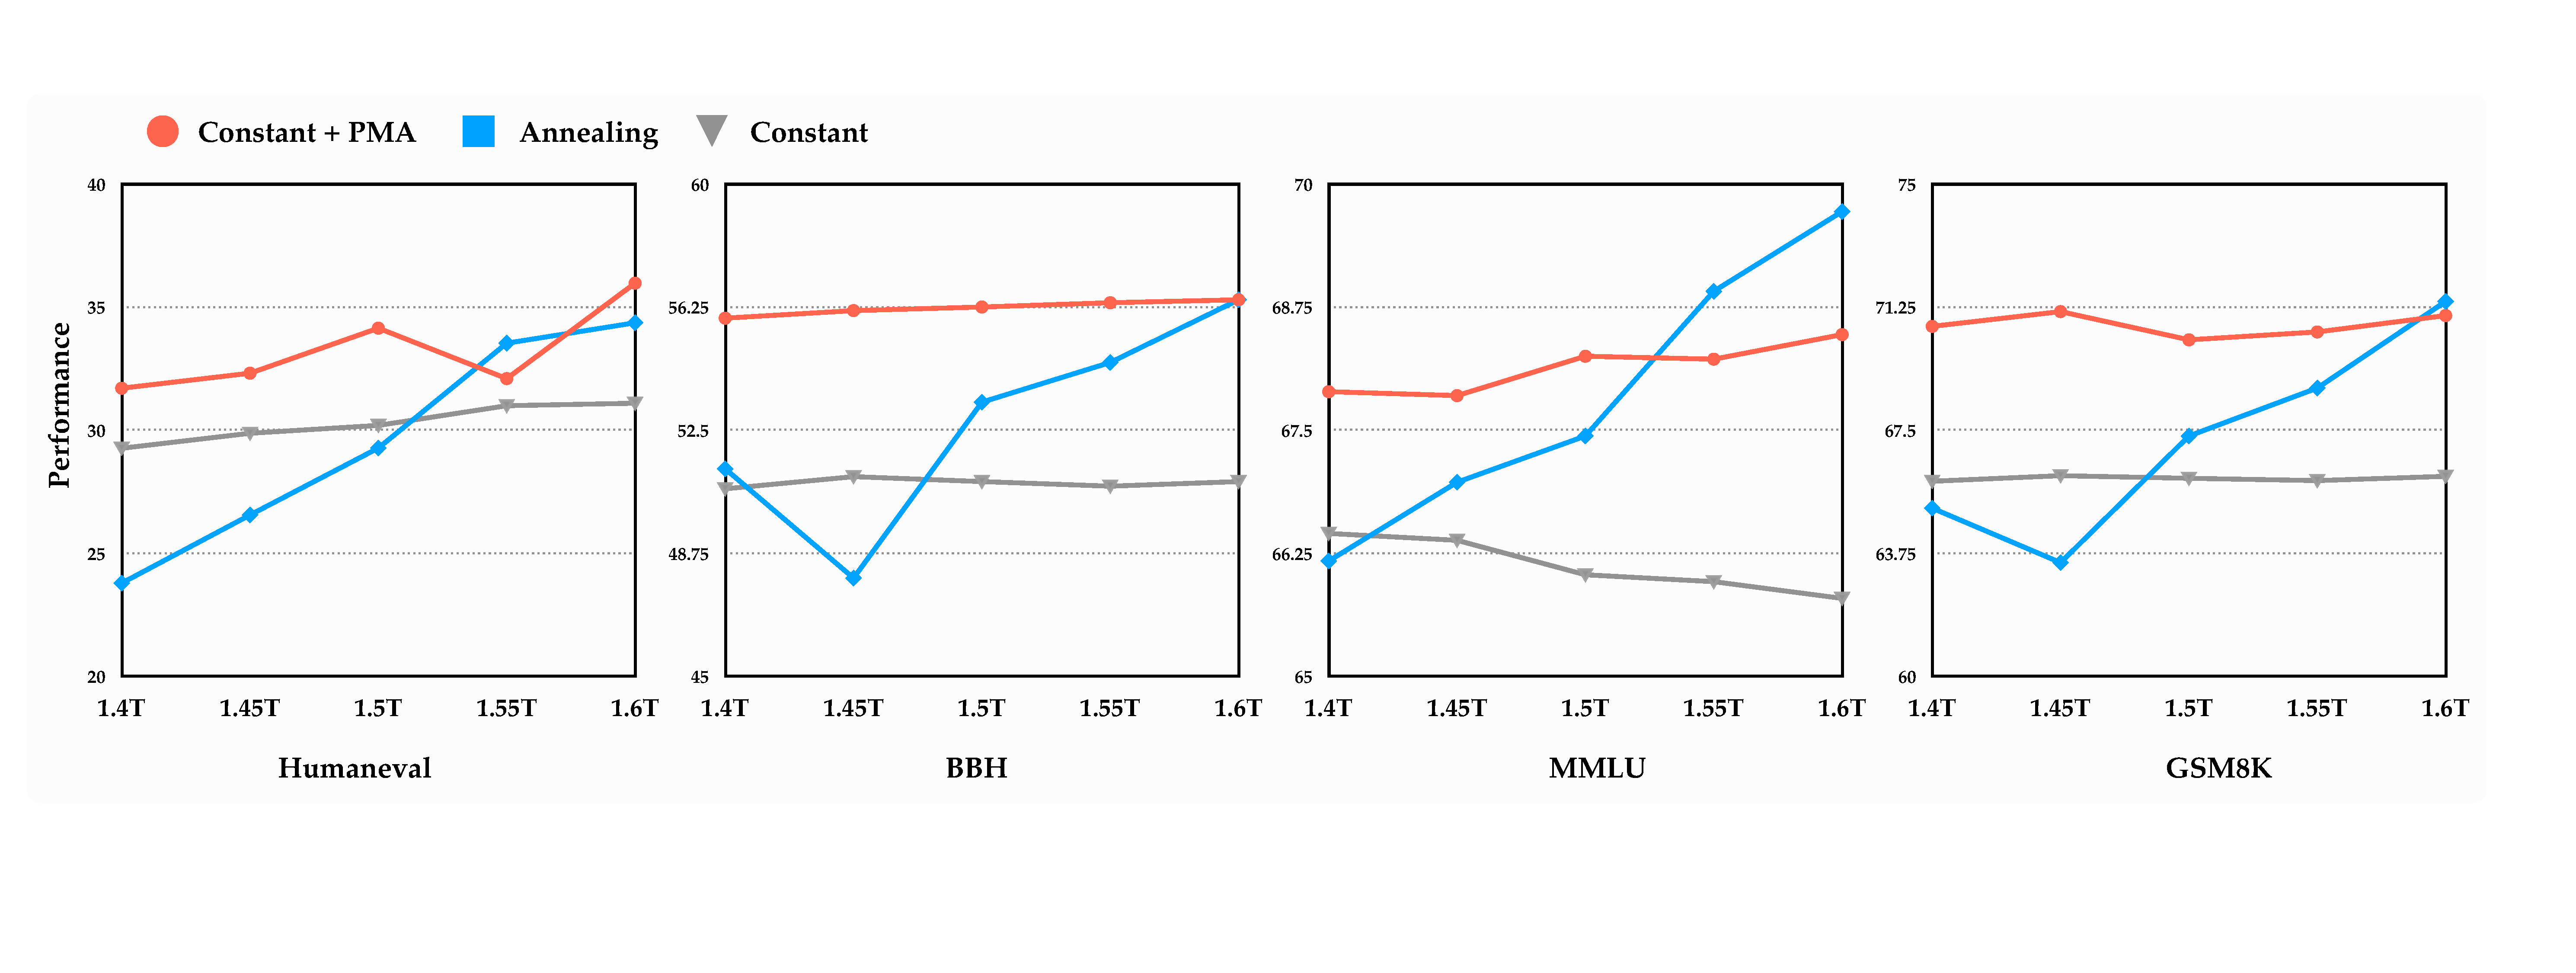
\includegraphics[width=1\linewidth]{image/cons_vs_aneal.pdf}
    \caption{Comparison of downstream task performance between model merging results under stable training and the real annealed model. The x-axis shows the count of training tokens.}
    \label{fig:cons_vs_aneal}
\end{figure}

\subsection{How do different merging methods affect final performance?}
\label{merging}
In this section, we systematically evaluate how different merging strategies affect the performance of merged models.
Specifically, we focus on three distinct approaches: EMA, WMA, and SMA.
% whether checkpoints with fewer training tokens should receive higher weights, checkpoints with more training tokens should be prioritized, or all checkpoints should be weighted equally. These approaches correspond to EMA, WMA, and SMA, respectively.
The EMA method employs exponentially decaying weights \(w_i = \alpha (1-\alpha)^{N-i}\),
giving higher importance to more recent checkpoints.
WMA assigns linearly increasing weights \(w_i = i\),
also prioritizing more recent checkpoints.
In contrast, SMA applies uniform weighting, treating all checkpoints equally regardless of their position in the training sequence.

\begin{figure}[t]
    \centering
    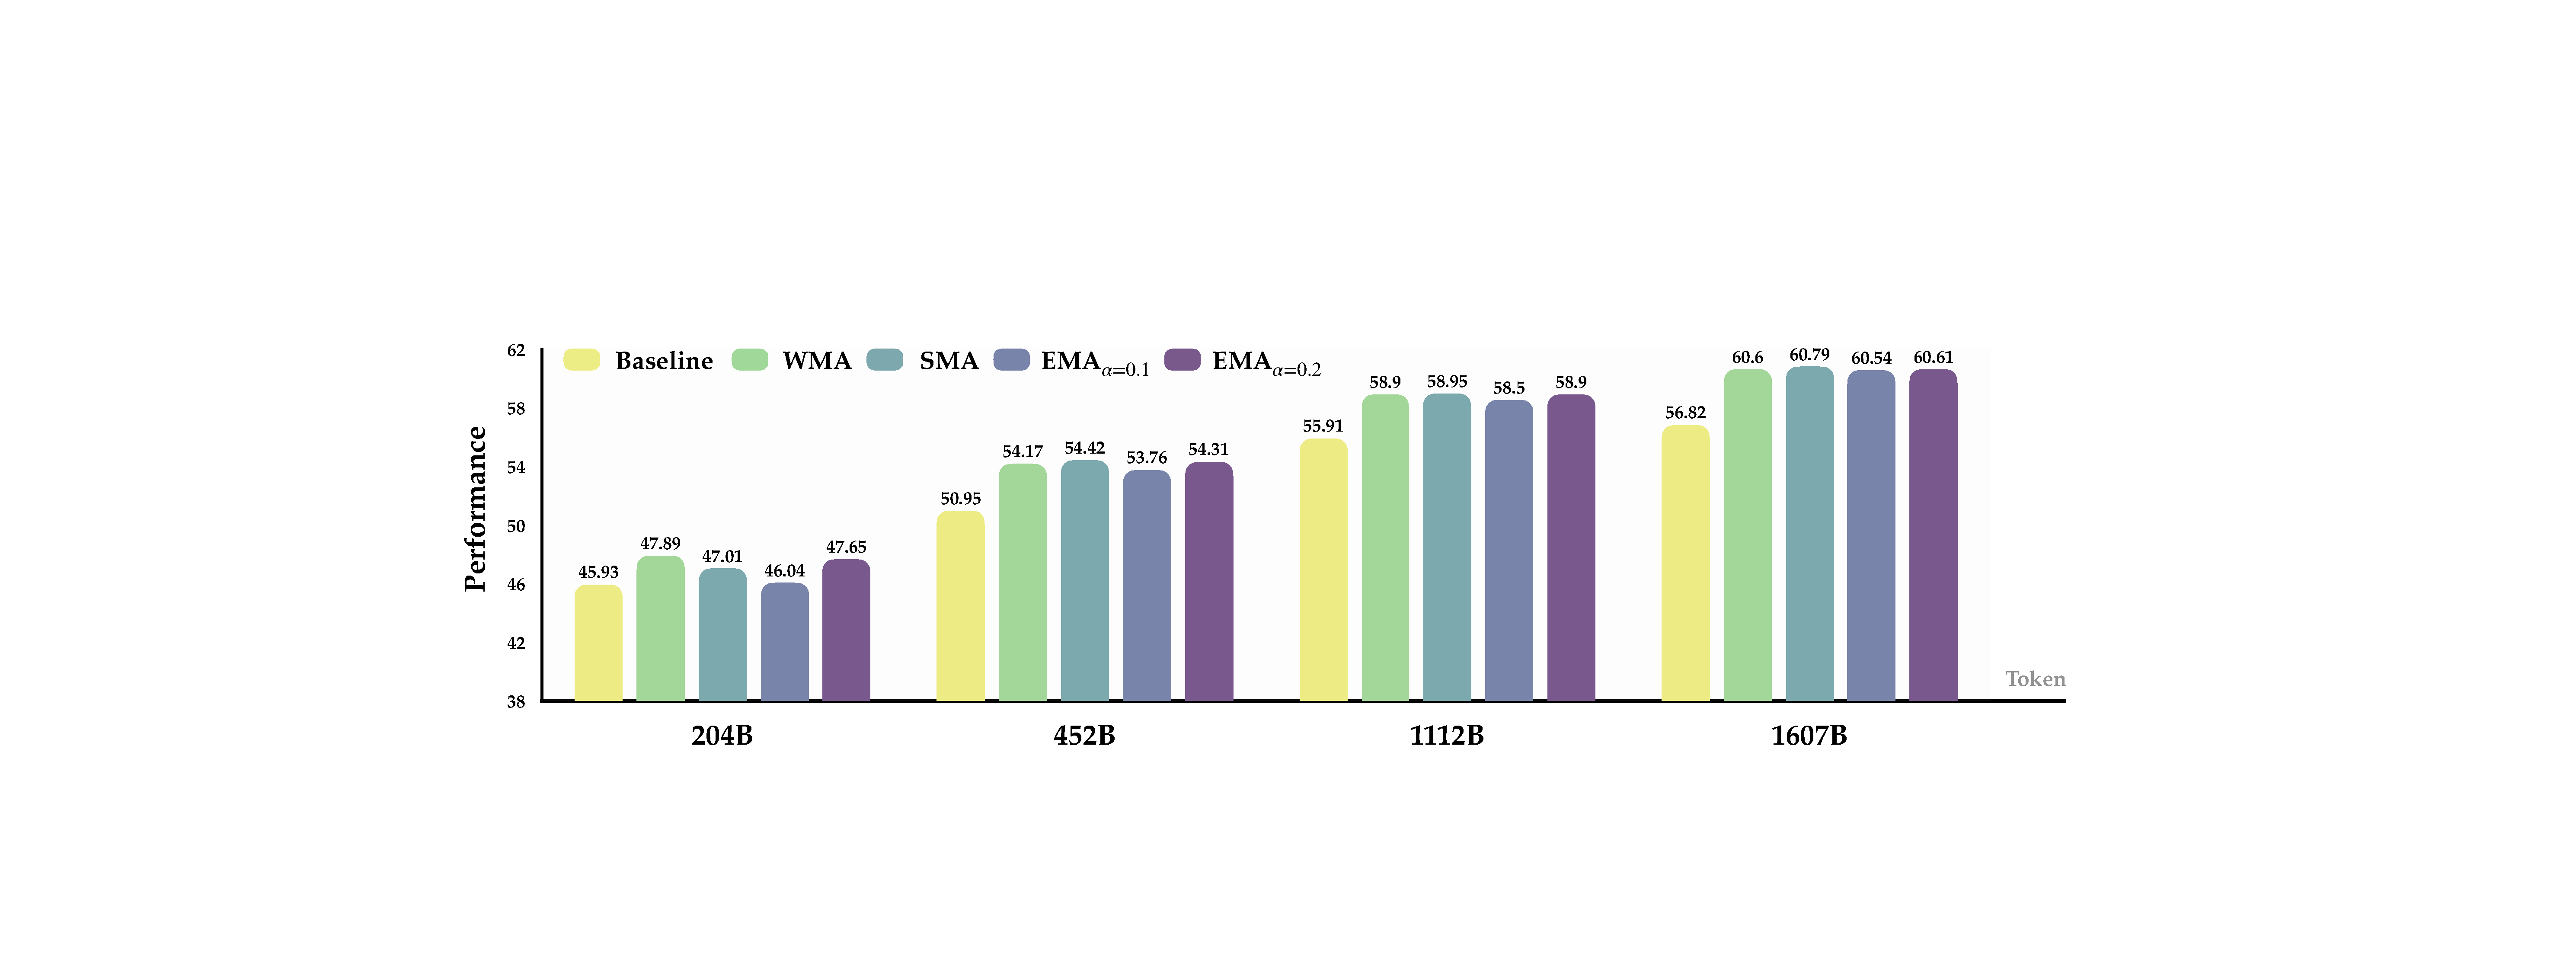
\includegraphics[width=1\linewidth]{image/mm_v.pdf}
    \caption{Impact of different model merging methods on final model performance.}
    \label{fig:mm_v}
\end{figure}

We conducted experiments on Seed-MoE-1.3/13B and showed the results in Figure~\ref{fig:mm_v}. At 204B training tokens, all merging methods enhanced model performance compared to the pre-merged model, but WMA delivered the best results. This suggests that in the early phases of training, when model weights undergo significant changes, assigning higher weights to checkpoints with more training tokens produces superior models. This is further supported by the fact that \(\text{EMA}_{\alpha=0.2}\) outperforms \(\text{EMA}_{\alpha=0.1}\). However, as training advances to later stages and model weights stabilize, the performance differences between merging methods diminish. For its simplicity and stability, we primarily use SMA for model merging in subsequent experiments.

\subsection{How to determine the optimal interval and
number of weights to merge for various model sizes?}
Beyond the merging technique itself, two other factors may also affect the effectiveness of model merging: the interval $V$ between selected models and the number of models $N$. We performed ablation studies on the Seed-MoE-1.3/13B model to investigate these effects, starting with the impact of the interval. As illustrated in the upper part of  Figure~\ref{fig:k_and_v}, we fixed $N=10$ and tested intervals of $V=4$B, 8B, 16B, and 32B. Notably, at 204B with $V=32$B, we reduced $N$ to 6 due to insufficient models. In the early stage of training, at 204B tokens, merged results with $V=16$B and $V=32$B underperformed the baseline. This is likely because large intervals incorporated unstable weights from the initial training phase, leading to significant weight disparities and suboptimal outcomes. As training progressed and weights stabilized, the performance gap across different $V$ settings gradually narrowed.
In practice, the optimal interval scales with model size, following these observed patterns: an interval of around 8B tokens for 1.3B/13B models, 4B tokens for 0.7B/7B models, and approximately 80B tokens for 10B/100B models. This aligns with the tendency of larger models to use larger batch sizes~\cite{mccandlish2018empirical}. 

Next, we set $V=8$B and explored how the number of merged models $N$ affects performance, testing $N=3$, 6, 10, and 15. As shown in the lower part of Figure~\ref{fig:k_and_v}, early in training, incorporating more models introduced unstable weights, which reduced the performance of merged models. However, once training was complete, merging a larger number of models led to significant performance improvements. Notably, the overall performance for $N=3$ was nearly 1 point lower than for $N=15$. To strike a balance between computational cost and performance gains, we opted for $N=10$ in further experiments.
\begin{figure}[h]
    \centering
    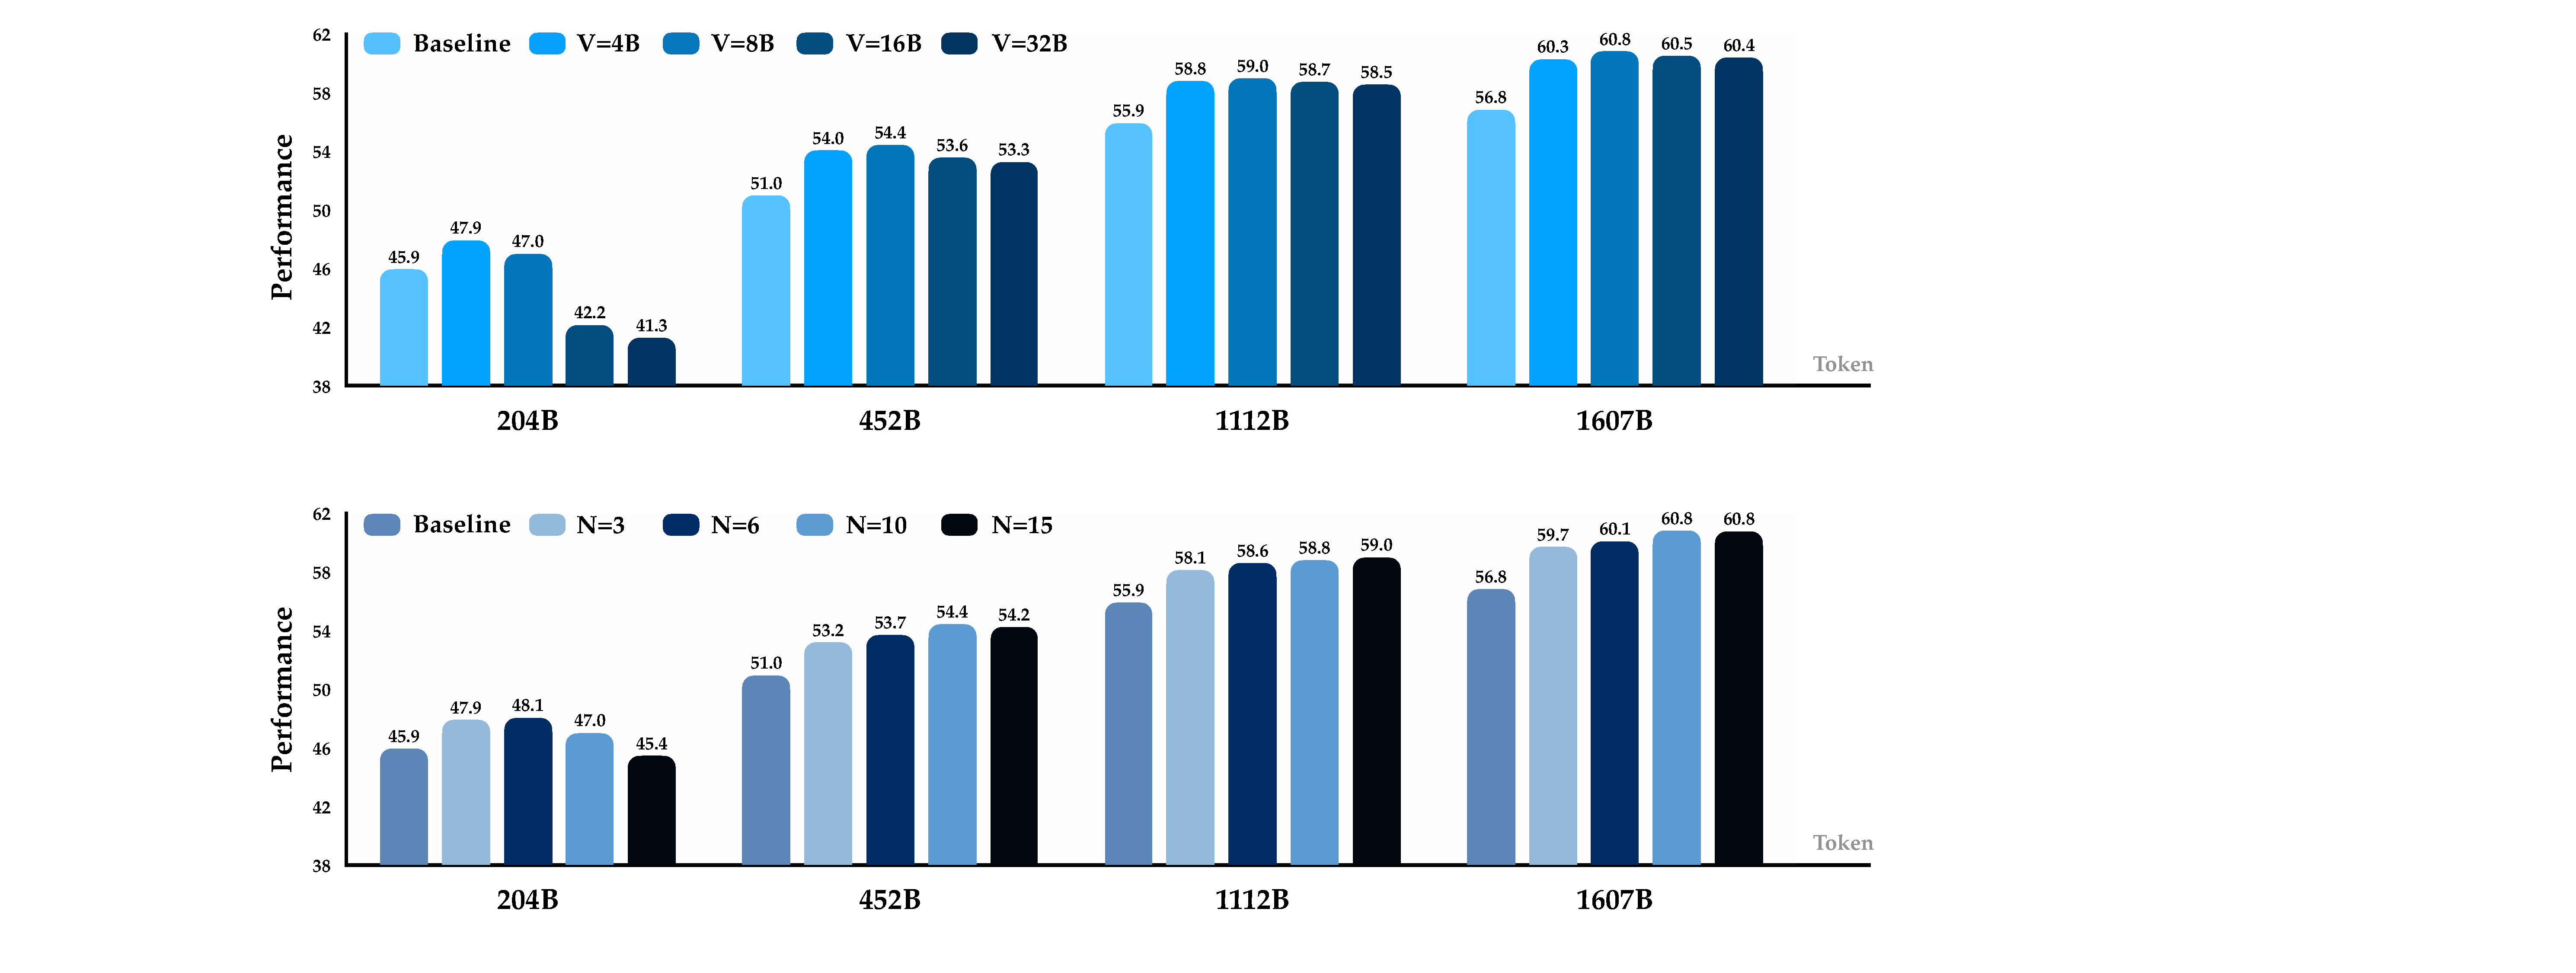
\includegraphics[width=0.9\linewidth]{image/k_and_v.pdf}
    \caption{Impact of different model merging hyper-parameters on final model performance.}
    \label{fig:k_and_v}
\end{figure}

\subsection{Do merged pre-trained models contribute to better downstream training?}
\label{4.4}
\begin{figure}
    \centering
    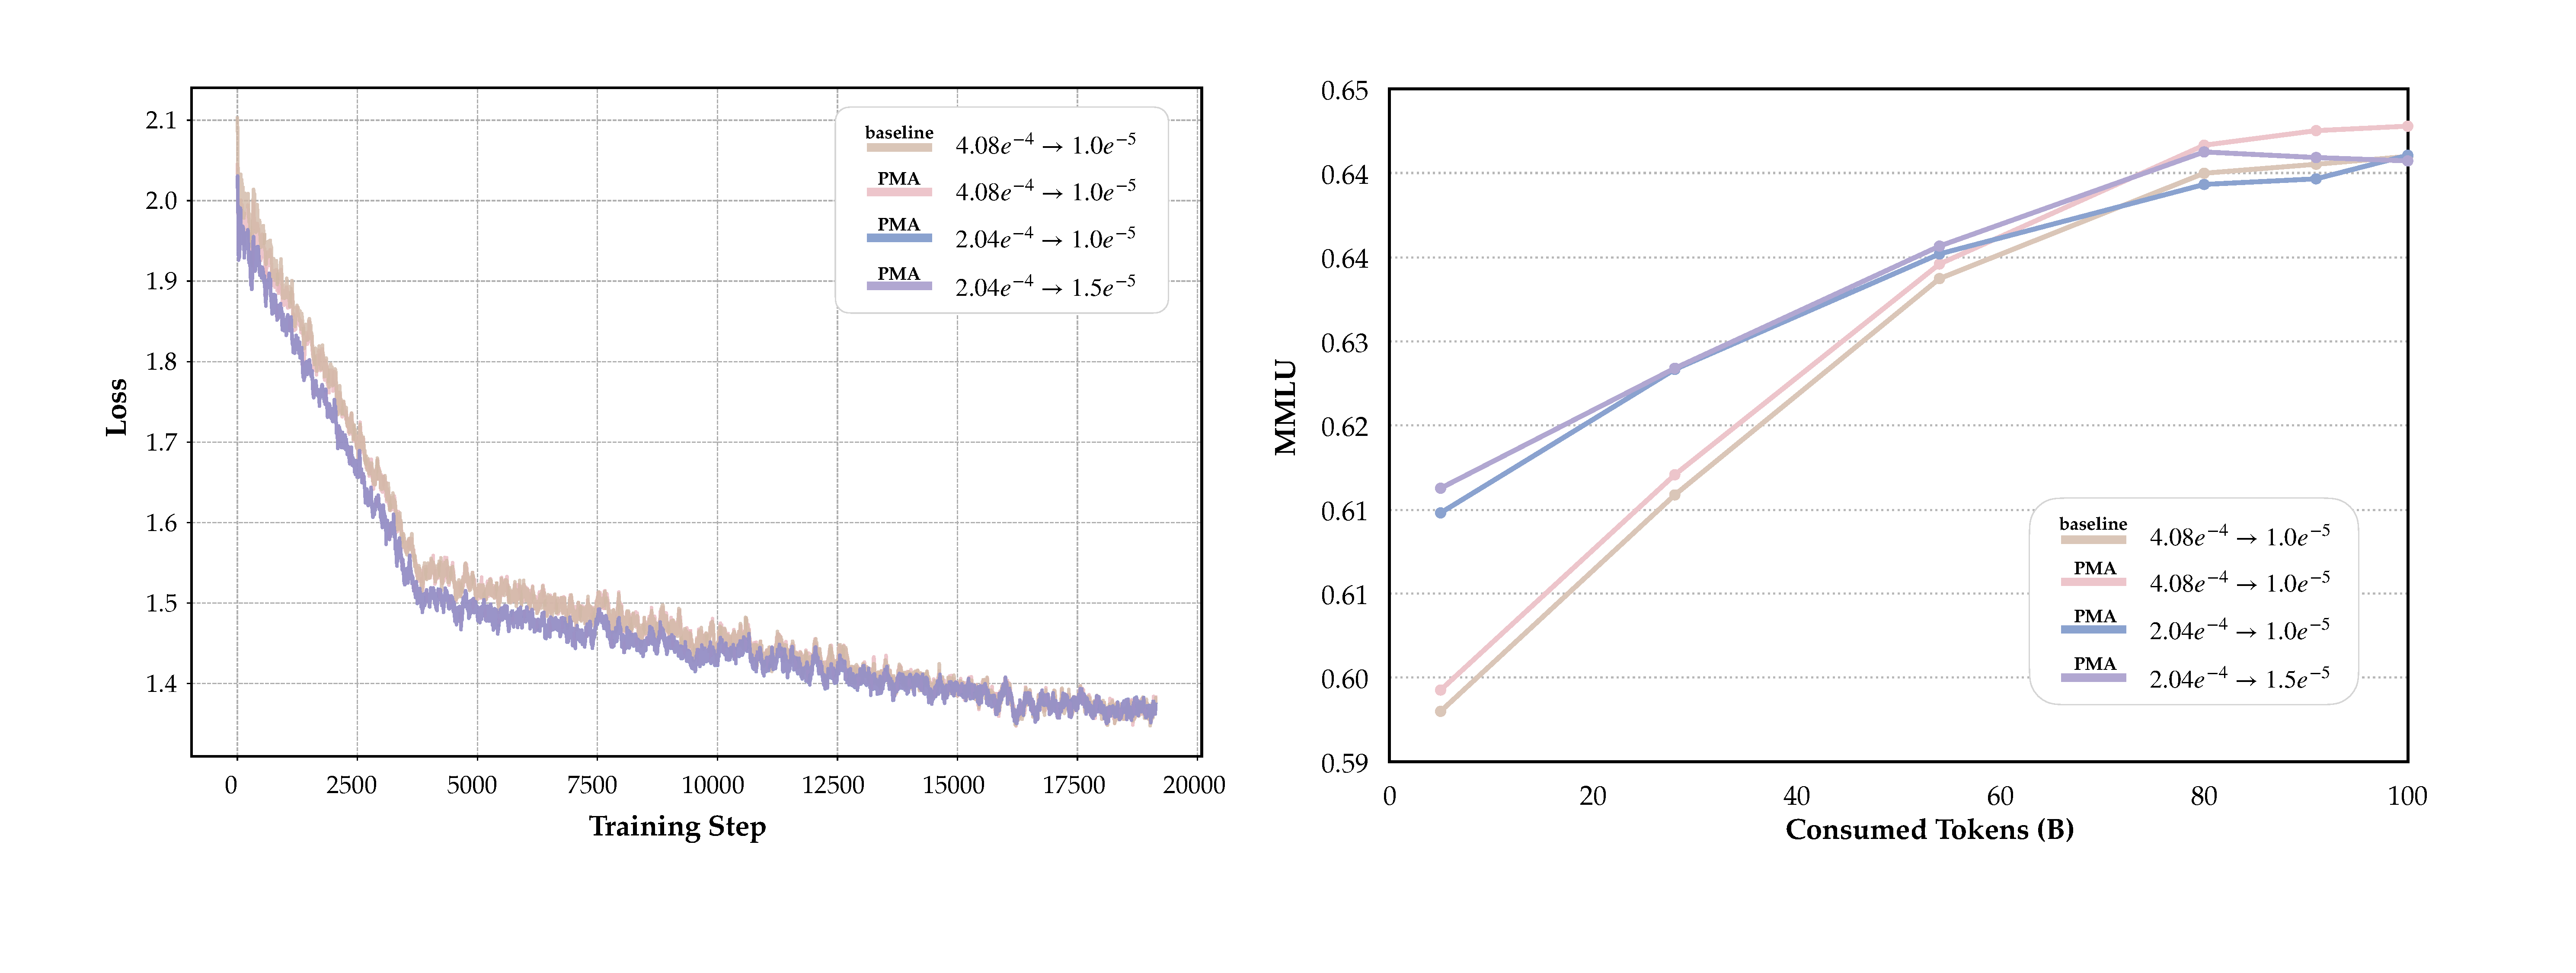
\includegraphics[width=0.9\linewidth]{image/merge_ct.pdf}
    \caption{Comparisons of loss curves (left) and performance metrics (right) during CT stage with varying $lr$ schedules, where a cosine scheduler is adopted to decay learning rate from $lr_{peak}$ to $lr_{end}$ (denoted as $lr_{peak} \rightarrow lr_{end}$). $\texttt{PMA}$ and $\texttt{baseline}$, stand for whether our \texttt{\OURS{}-init} technique is employed or not, respectively.} %\CY{curves are not obvious in left (pink and blue)}}
    \label{fig:merge_ct}
\end{figure}

A complete LLM training process typically involves multiple stages, which are pretraining, continual training (CT), supervised fine-tuning (SFT) and reinforcement learning (RL) in sequence.
In light of the capacity of \OURS{} to improve pretraining performance, we conjecture that merged pretrained models may similarly prove beneficial for downstream stages.
To verify this hypothesis, we initialized downstream training with \OURS{}, which we dubbed as \texttt{\OURS{}-init}, and investigated its impacts over the baselines (which are initialized from their original checkpoints) for both CT and SFT stages.


\textbf{CT stage.}
We first conducted an ablation study to assess the sensitivity of the \texttt{\OURS{}-init} of the CT stage with varying learning rate schedules.
Specifically, we experimented with Seed-MoE-0.7B/7B models merged after stable training on approximately 1 trillion tokens. 
As illustrated in Figure~\ref{fig:merge_ct} (left), the initialization weights obtained via \OURS{} consistently achieved marginally lower loss at the initial training phase, against the baseline with the same training configuration. 
As training progresses, the loss values for models with different initialization weights converge to comparable levels. 
It's worth noting that in the loss curve, the purple line significantly overlaps with the blue line, and the brown line significantly overlaps with the pink line.
% \CY{"different initialization weights", or "different training configurations (lr)"?}
Another observation is made in the Figure~\ref{fig:merge_ct} (right), where evaluation on the MMLU benchmark reveals that the \texttt{\OURS{}-init} models outperform the baseline early in training. While these models tend to retain a slight performance edge in later stages, their results on other tasks may be slightly suboptimal, leading to overall performance parity with the baseline. Experiments across varied learning rate schedules corroborate these findings, indicating that models converge to similar performance levels by the end of training, and no extensive learning rate tuning is required for \texttt{\OURS{}-init}. 
% \CY{it seems only one PMA run achieves distinctly better result than baseline, while for the rest two runs, their early-stage advance was eventually caught up by the beseline. Shall we mention this? Does it reduce our impact?}

\textbf{SFT stage.}
We next analyzed the impact of \texttt{\OURS{}-init} on the SFT stage, where the detailed results can be found in the Appendix~\ref{app-sft}. 
Although initialization with merged weights occasionally yields performance improvements, such gains are not consistently observed. 
Nonetheless, this approach does not adversely affect downstream training outcomes and may be a viable strategy for researchers seeking to enhance model performance.


\subsection{Does model merging improve the training stability?}
In large-scale LLM training, infrastructure issues are almost inevitable and often lead to training instability phenomena such as loss spikes or diverging.
Specifically, a loss spike occurs when, at a specific point during the multi-stage training, the model's predictions deteriorate significantly compared to previous iterations. 
This phenomenon is often observed alongside gradient norm (GradNorm) explosion during backpropagation, which causes large weight updates and eventually lead to a irrecoverable spike in its loss function~\cite{cohen2021gradient}. 
In the experiments detailed in Section~\ref{4.4}, as illustrated in Figure~\ref{fig:resume} (left), we observed that a model initialized with \texttt{\OURS{}-init} for SFT stage demonstrated a notably more stable GradNorm metric compared to the baseline. This stability is also evident in the reduced frequency of loss spikes relative to the baseline. 
Since applying \texttt{\OURS{}-init} for downstream training does not impact the model's final performance and remains robust across different learning rates, we established a series of experiments to explore whether model merging could enhance training stability. 

% \textbf{Pre-training stage.} 
Given the extremely high expenses associated, it is unfeasible to conduct a direct analysis of training instability in LLM pre-training. 
Experiments~\cite{wortsman2023small} show that small models using a relatively large learning rate will exhibit unstable training characteristics similar to those of large models. 
We thus reproduce the instability phenomena on small models to study the influence of our \texttt{\OURS{}-init} on training stability.
In one such experiment, we trained a 330M/3.3B MoE model from scratch using an exceptionally high learning rate of 6e-3. 
As shown in Figure~\ref{fig:resume} (right), the model overshot the optimal weights, resulting in unstable training and abrupt loss spikes as expected, and was irreversible to its original trajectory. 
To address this, we adopted \texttt{\OURS{}-init} with three checkpoints saved before the training collapse happened, to resume the pre-training process. As depicted by the red line in Figure~\ref{fig:resume} (right), the resumed training process stabilized, successfully navigating past the point of the loss spike and continuing along its original training trajectory.

% \textbf{SFT stage.} In the experiments detailed in Section~\ref{4.4}, as illustrated in Figure~\ref{fig:resume} (left), we observed that a model initialized with \texttt{\OURS{}-init} for SFT stage demonstrated a notably more stable GradNorm metric compared to the baseline. This stability is also evident in the reduced frequency of loss spikes relative to the baseline. \CY{If you agree with this presentation order change (pretraining -> SFT), maybe we shall swith the left and right in Fig.7 :)}

These results highlight that \texttt{\OURS{}-init} can reliably enhance the multi-stage training stability.
When a loss spike occurs, one can merge the model checkpoints from before the spike and resume training from that point. 
This approach provides an alternative solution to avoid retraining the model from scratch, thereby substantially reducing the waste of computational resources.

\begin{figure}
    \centering
    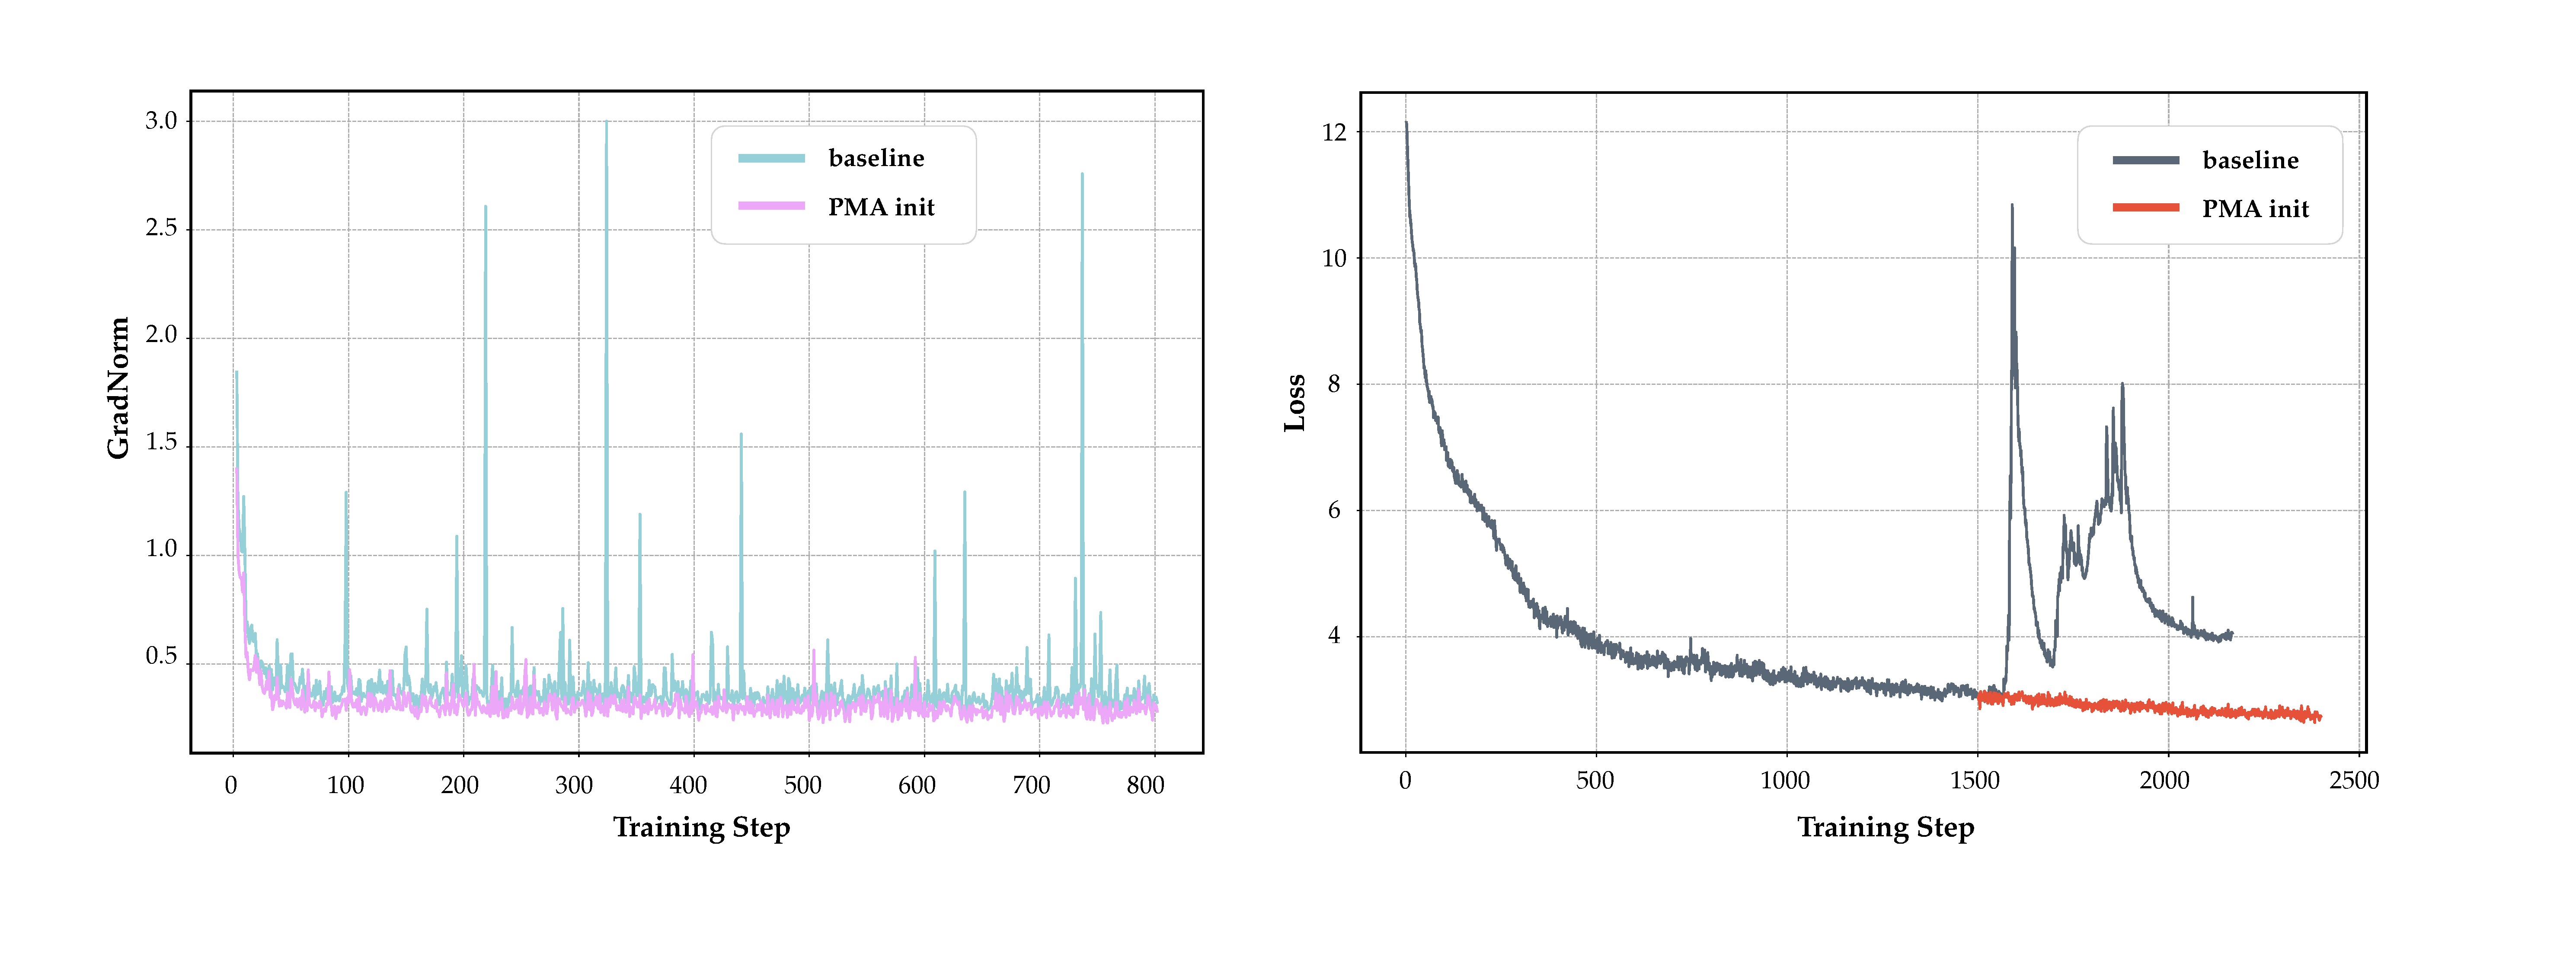
\includegraphics[width=0.9\linewidth]{image/resume.pdf}
    \caption{Left: GradNorm comparisons for SFT training initialized with \texttt{\OURS{}-init}. Right: Comparison of pre-training loss curves between resuming with \texttt{\OURS{}-init} and the original training.}
    \label{fig:resume}
\end{figure}
% \subsection{What processes unfold during model merging?}
% To gain deeper insight into the mechanisms behind model merging, we offer both qualitative and quantitative analyses through mathematical proofs and visualizations of the weights.

% We perform a second-order Taylor expansion of the loss function \(L(\theta)\) around the optimal parameter \(\theta^*\):
% \[
% L(\theta) \approx L(\theta^*) + \underbrace{(\theta - \theta^*)^T \nabla L(\theta^*)}_{\text{=0, as }\theta^*\text{ is optimal.}} + \frac{1}{2}(\theta - \theta^*)^T H (\theta - \theta^*)
% \]
% where \(H\) is the Hessian matrix of the loss function at \(\theta^*\) (the matrix of second derivatives), representing curvature information. Since \(\theta^*\) is the optimal point, the first derivative is zero, simplifying to:
% \[
% L(\theta) \approx L(\theta^*) + \frac{1}{2}(\theta - \theta^*)^T H (\theta - \theta^*)
% \]
% Assume we have \(k\) model parameters \(\theta_1, \theta_2, ..., \theta_k\), and define the deviation vector of each model from the optimal parameter as \(\delta_i = \theta_i - \theta^*\).
% The loss estimate for each model \(i\) is given by:
% \[
% L(\theta_i) \approx L(\theta^*) + \frac{1}{2}\delta_i^T H \delta_i
% \]
% The average loss of all individual models is:
% \[
% \frac{1}{k}\sum_{i=1}^k L(\theta_i) \approx L(\theta^*) + \frac{1}{2k}\sum_{i=1}^k \delta_i^T H \delta_i
% \]
% The merged parameter is defined as: \(\theta_{avg} = \frac{1}{k}\sum_{i=1}^k \theta_i\).
% The deviation of the merged model from the optimal parameter is: \(\theta_{avg} - \theta^* = \frac{1}{k}\sum_{i=1}^k \delta_i\).
% The loss estimate for the merged model is:
% \[
% L(\theta_{avg}) \approx L(\theta^*) + \frac{1}{2}\left(\frac{1}{k}\sum_{i=1}^k \delta_i\right)^T H \left(\frac{1}{k}\sum_{i=1}^k \delta_i\right)
% \]
% Expanding this gives:
% \[
% \frac{1}{2}\left(\frac{1}{k}\sum_{i=1}^k \delta_i\right)^T H \left(\frac{1}{k}\sum_{i=1}^k \delta_i\right) = \frac{1}{2k^2}\sum_{i=1}^k\sum_{j=1}^k \delta_i^T H \delta_j
% \]
% This can be rewritten as:
% \[
% \frac{1}{2k^2}\left(\sum_{i=1}^k \delta_i^T H \delta_i + \sum_{i=1}^k\sum_{j\neq i} \delta_i^T H \delta_j\right)
% \]
% The condition for the loss of the merged model to be less than the average loss is:
% \[
% \frac{1}{2k^2}\left(\sum_{i=1}^k \delta_i^T H \delta_i + \sum_{i=1}^k\sum_{j\neq i} \delta_i^T H \delta_j\right) < \frac{1}{2k}\sum_{i=1}^k \delta_i^T H \delta_i
% \]
% Simplifying gives:
% \[
% \sum_{i=1}^k\sum_{j\neq i} \delta_i^T H \delta_j < (k-1)\sum_{i=1}^k \delta_i^T H \delta_i
% \]
%  When \(H\) is a positive definite matrix (which is usually the case since we are seeking a minimum), \(\delta_i^T H \delta_i > 0\).
% When the deviation vectors of different models are "negatively correlated" in the loss landscape, i.e., most \(\delta_i^T H \delta_j < 0 (i \neq j)\), the above inequality becomes easier to satisfy.

% This mathematical relationship can be intuitively understood as follows:
% 1. The effectiveness of merging model weights arises from the fact that different models explore different directions in the parameter space.
% 2. When these directions exhibit a certain "complementarity" in the geometric structure of the loss function, their average can be closer to the optimal point.
% 3. This explains why merging models during training often improves performance.
% This analysis reveals that weight merging is not simply averaging parameters but rather leverages the geometric structure of the parameter space and the complementary nature of different models.

% \begin{figure}[h]
%     \centering
%     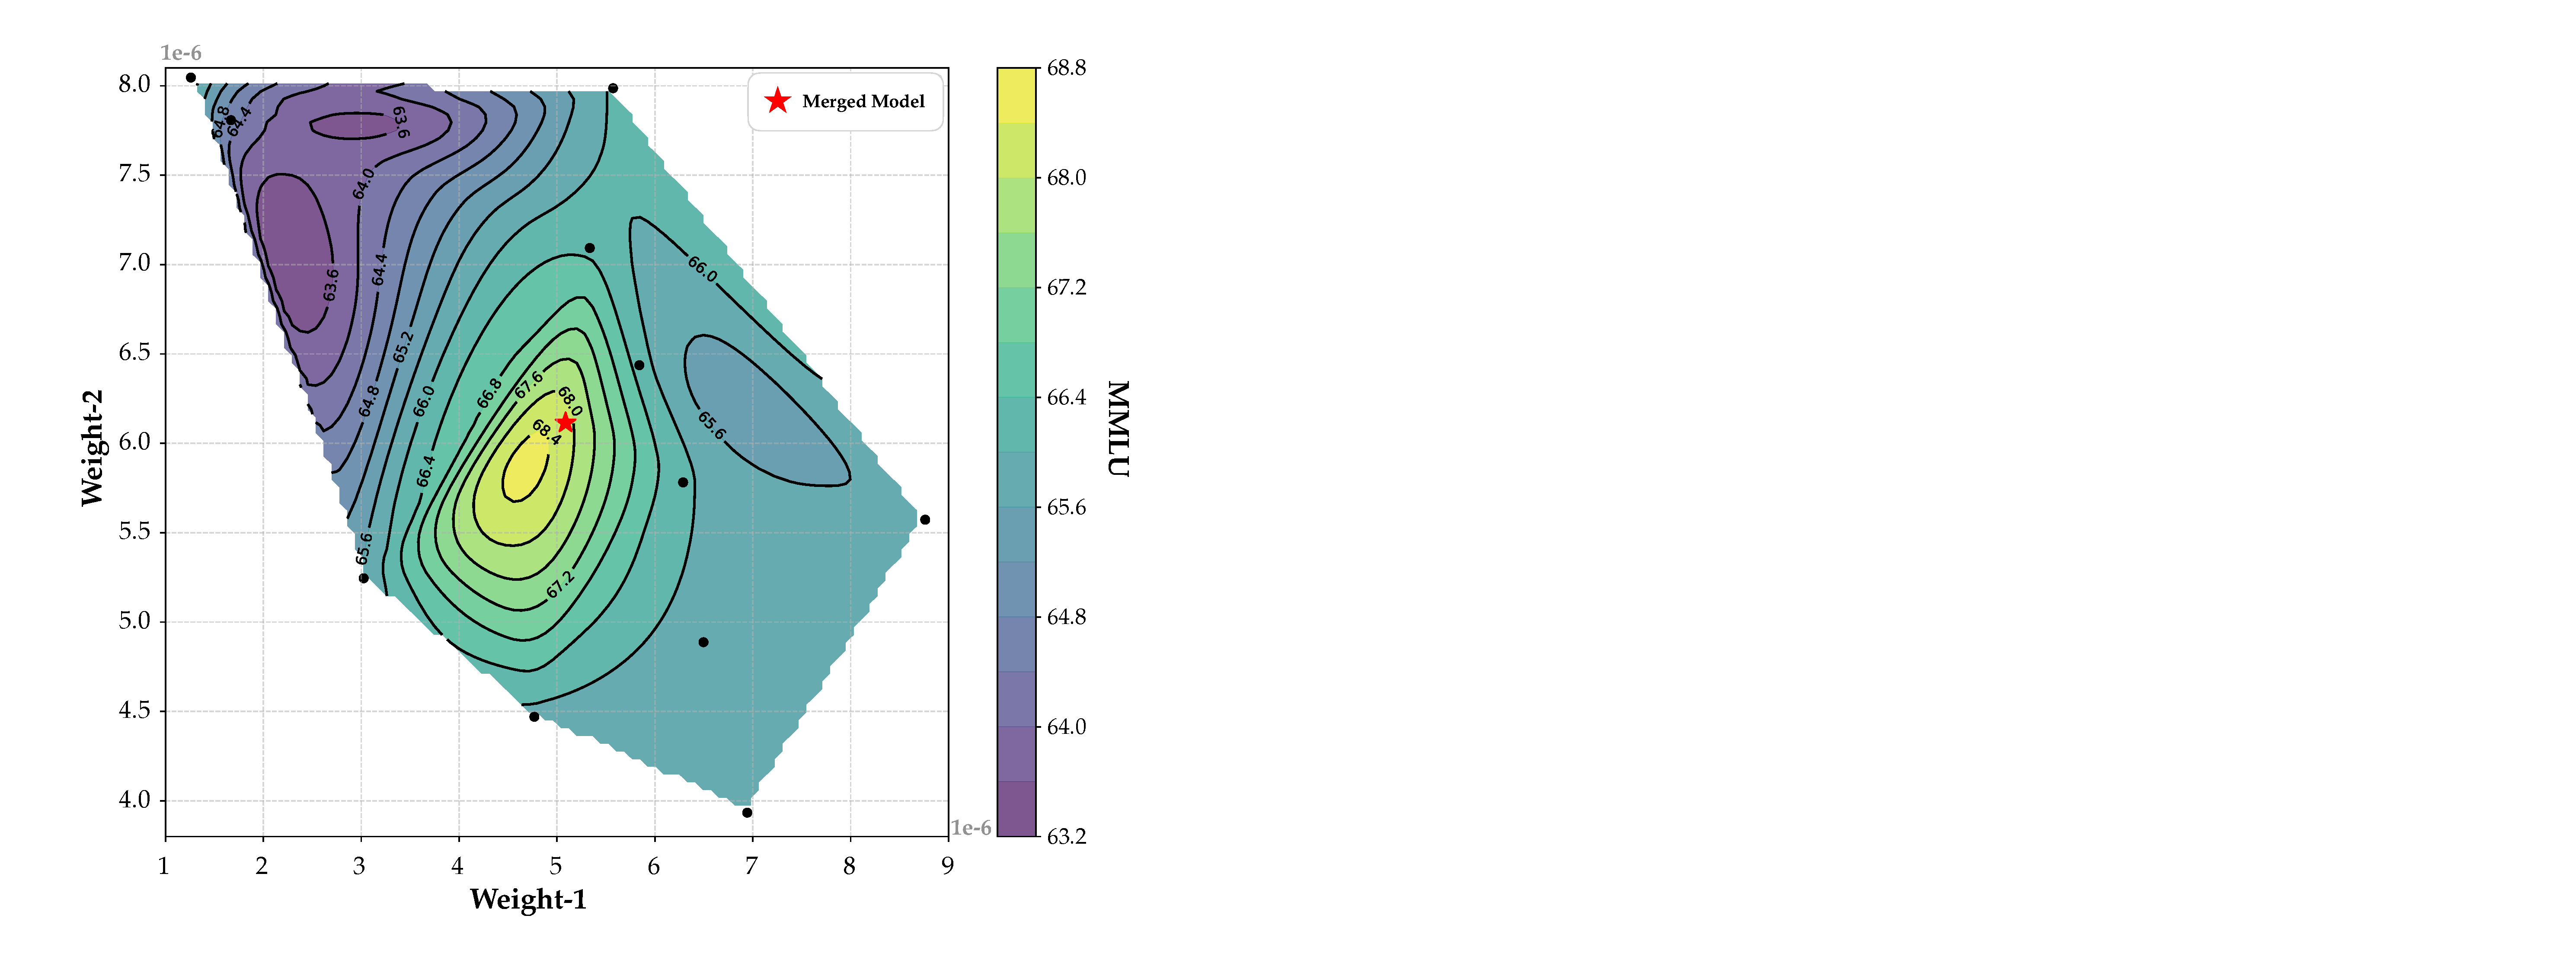
\includegraphics[width=0.6\linewidth]{image/keshihua.pdf}
%     \caption{Visualization of contour lines representing MMLU scores, comparing the weights of the original model with those of the merged model.}
%     \label{fig:keshihua}
% \end{figure}
% Additionally, we selected several checkpoints from the pre-training of Seed-MoE-1.3B/13B and visualized the average distribution of two parameters in a specific layer. Using these points, we generated contour lines for MMLU scores, as illustrated in Figure~\ref{fig:keshihua}, with the weight positions of various models marked as black dots. These dots are distributed along the MMLU score contours, revealing a notable "complementary" pattern. The average weight position is closer to the optimal minimum than that of individual models. This figure also clearly explains why model merging yields less improvement when annealed to a very low learning rate compared to merging at a higher learning rate. At a low learning rate, the models to be merged are already stuck in a local optimum, and even after merging, they remain trapped in this suboptimal region, unable to reach a more optimal solution.

\subsection{Investigating the Mechanisms of Model Merging}
\label{subsec:merging_mechanisms}

To gain deeper insight into the underlying mechanisms that enable model merging to be effective, we provide both qualitative and quantitative analyses, employing mathematical derivations and visualizations of weight distributions.

We begin with a second-order Taylor expansion of the loss function \(L(\theta)\) around an optimal parameter set \(\theta^*\):
\begin{equation}
L(\theta) \approx L(\theta^*) + (\theta - \theta^*)^T \nabla L(\theta^*) + \frac{1}{2}(\theta - \theta^*)^T H (\theta - \theta^*),
\end{equation}
where \(H\) is the Hessian matrix of the loss function evaluated at \(\theta^*\) (the matrix of second partial derivatives), which captures curvature information. Since \(\theta^*\) is an optimal point, the gradient \(\nabla L(\theta^*)\) is zero. Thus, the expansion simplifies to:
\begin{equation}
L(\theta) \approx L(\theta^*) + \frac{1}{2}(\theta - \theta^*)^T H (\theta - \theta^*).
\end{equation}
Consider \(k\) sets of model parameters \(\theta_1, \theta_2, \ldots, \theta_k\). Let the deviation vector of each model \(i\) from the optimal parameters be \(\delta_i = \theta_i - \theta^*\). The loss for each model \(i\) can then be approximated as:
\begin{equation}
L(\theta_i) \approx L(\theta^*) + \frac{1}{2}\delta_i^T H \delta_i .
\end{equation}
The average loss of these \(k\) individual models is:
\begin{equation}
\frac{1}{k}\sum_{i=1}^k L(\theta_i) \approx L(\theta^*) + \frac{1}{2k}\sum_{i=1}^k \delta_i^T H \delta_i .
\end{equation}
The parameters of the merged model are \(\theta_{\text{avg}} = \frac{1}{k}\sum_{i=1}^k \theta_i\). The deviation of this merged model from the optimal parameters is \(\theta_{\text{avg}} - \theta^* = \frac{1}{k}\sum_{i=1}^k \delta_i\).
The loss for the merged model is approximated by:
\begin{equation}
L(\theta_{\text{avg}}) \approx L(\theta^*) + \frac{1}{2}\left(\frac{1}{k}\sum_{i=1}^k \delta_i\right)^T H \left(\frac{1}{k}\sum_{i=1}^k \delta_i\right)
\end{equation}
Expanding the quadratic term:
\begin{equation}
\frac{1}{2}\left(\frac{1}{k}\sum_{i=1}^k \delta_i\right)^T H \left(\frac{1}{k}\sum_{i=1}^k \delta_i\right) = \frac{1}{2k^2}\sum_{i=1}^k\sum_{j=1}^k \delta_i^T H \delta_j .
\end{equation}
This can be rewritten by separating diagonal and off-diagonal terms:
\begin{equation}
\frac{1}{2k^2}\left(\sum_{i=1}^k \delta_i^T H \delta_i + \sum_{i=1}^k\sum_{j\neq i} \delta_i^T H \delta_j\right).
\end{equation}
For the merged model to have a lower loss than the average loss of the individual models, i.e., \(L(\theta_{\text{avg}}) < \frac{1}{k}\sum_{i=1}^k L(\theta_i)\), the following condition must hold:
\begin{equation}
\frac{1}{2k^2}\left(\sum_{i=1}^k \delta_i^T H \delta_i + \sum_{i=1}^k\sum_{j\neq i} \delta_i^T H \delta_j\right) < \frac{1}{2k}\sum_{i=1}^k \delta_i^T H \delta_i.
\end{equation}
Multiplying by \(2k^2\) and rearranging terms, we get:
\begin{equation}
\sum_{i=1}^k \delta_i^T H \delta_i + \sum_{i=1}^k\sum_{j\neq i} \delta_i^T H \delta_j < k\sum_{i=1}^k \delta_i^T H \delta_i.
\end{equation}
Which simplifies to:
\begin{equation}
\sum_{i=1}^k\sum_{j\neq i} \delta_i^T H \delta_j < (k-1)\sum_{i=1}^k \delta_i^T H \delta_i
\end{equation}
Assuming \(H\) is a positive definite matrix (which is generally true around a local minimum), then each term \(\delta_i^T H \delta_i > 0\). The inequality is more easily satisfied if the off-diagonal terms \(\delta_i^T H \delta_j\) (for \(i \neq j\)) are predominantly negative. This "negative correlation" in the context of the Hessian means that the deviation vectors point in somewhat opposing directions relative to the curvature of the loss landscape.
\begin{figure}[h]
    \centering
    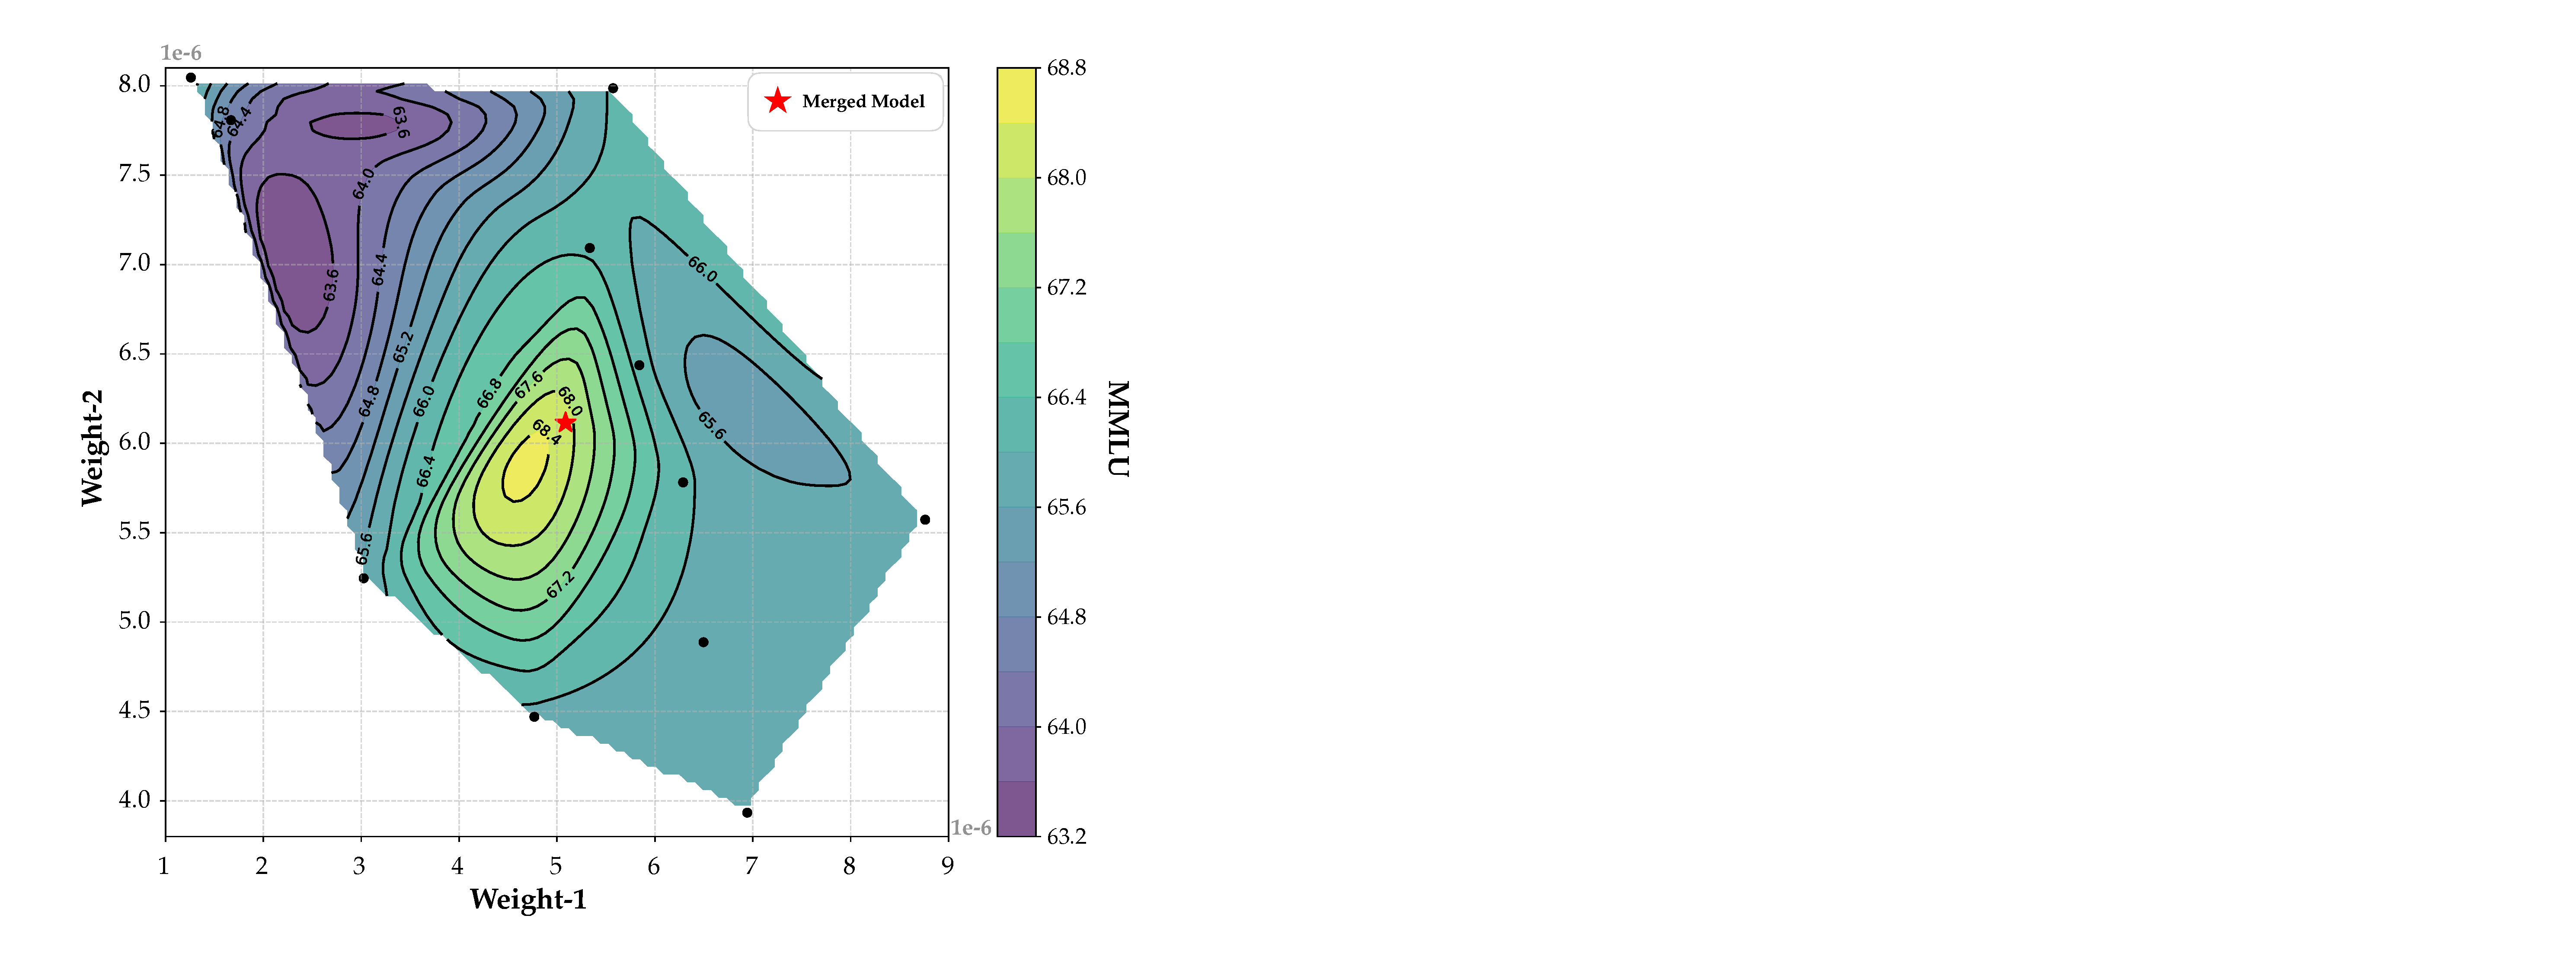
\includegraphics[width=0.6\linewidth]{image/keshihua.pdf}
    \caption{Visualization of MMLU score contour lines, comparing the weights of an original model with those of a merged model. Black dots represent the parameter locations of various individual model checkpoints.}
    \label{fig:keshihua}
\end{figure}
This mathematical analysis can be intuitively interpreted as follows:
1.  The effectiveness of model weight merging stems from the fact that different model checkpoints, representing different points in the training trajectory, have explored different local regions or directions within the parameter space.
2.  When these explorations exhibit a degree of "complementarity" concerning the geometric structure of the loss function (captured by the Hessian and the cross-terms \(\delta_i^T H \delta_j\)), their average can position the merged model closer to an optimal point than the individual models might be on average.
3.  This helps explain why merging models, particularly those from a stable yet ongoing training phase, often improves performance. The averaging process can smooth out idiosyncrasies of individual checkpoints.
This analysis suggests that weight merging is not merely a simple averaging of parameters but rather a process that can leverage the geometric structure of the loss landscape and the diversity among the models being merged.

Additionally, we selected several checkpoints from the pre-training of Seed-MoE-1.3B/13B and visualized the average distribution of two selected parameters from a specific layer. Using these points, we generated contour lines for MMLU scores, as illustrated in Figure~\ref{fig:keshihua}. The weight positions of various individual models are marked as black dots. These dots are distributed along the MMLU score contours, revealing a discernible "complementary" pattern. The averaged weight position (representative of the merged model) is often situated closer to a region of higher MMLU scores (a better optimum) than many individual model checkpoints. This visualization also provides an intuitive explanation for why model merging yields diminished improvements when models are annealed to a very low learning rate: at such a stage, the models to be merged are already tightly converged within a specific local optimum. Merging them essentially averages points within this already narrow basin, making it unlikely to escape to a significantly better or different optimal region.
